%%%%%%%%%%%%%%%%%%%%%%%%%%%%%%%%%%%%%%%%%%%%%%%%%%%%%%%%%%%%%%%%%%%%%%
% How to use writeLaTeX: 
%
% You edit the source code here on the left, and the preview on the
% right shows you the result within a few seconds.
%
% Bookmark this page and share the URL with your co-authors. They can
% edit at the same time!
%
% You can upload figures, bibliographies, custom classes and
% styles using the files menu.
%
%%%%%%%%%%%%%%%%%%%%%%%%%%%%%%%%%%%%%%%%%%%%%%%%%%%%%%%%%%%%%%%%%%%%%%

\documentclass[12pt]{article}

\usepackage{sbc-template}

\usepackage{graphicx,url}

%\usepackage[brazil]{babel}   
\usepackage[utf8]{inputenc} 

\usepackage{float}
\usepackage{hyperref}

\usepackage{listings}
\usepackage{color}

\definecolor{dkgreen}{rgb}{0,0.6,0}
\definecolor{gray}{rgb}{0.5,0.5,0.5}
\definecolor{mauve}{rgb}{0.58,0,0.82}

\lstset{frame=none,
  language=C++,
  aboveskip=3mm,
  belowskip=3mm,
  showstringspaces=false,
  columns=flexible,
  basicstyle={\small\ttfamily},
  numbers=none,
  numberstyle=\tiny\color{gray},
  keywordstyle=\color{blue},
  commentstyle=\color{dkgreen},
  stringstyle=\color{mauve},
  breaklines=true,
  breakatwhitespace=true,
  tabsize=3
}

     
\sloppy

\title{MQTT}

\author{Fabricio Araújo Dias}

\address{Instituto Federal de Educação, Ciência e Tecnologia do Ceará
  (IFCE)\\
  Avenida Vice-Presidente José Alencar, S/N -- 61.939-140 -- Maracanaú -- CE -- Brasil
  \email{fabricio.araujo61@aluno.ifce.edu.br}
}

\begin{document} 

\maketitle

\begin{abstract}
    Report about the eighth Microcontroller practical activity which demonstrates the use of the MQTT protocol to send and receive messages on the ESP32. To test this, the messages received will be printed on the monitor or will change the state of an RGB LED.
\end{abstract}
     
\begin{resumo} 
    Relatório sobre a oitava atividade prática de Microcontrolares que provê demonstrar o uso do protocolo \textit{MQTT} para o envio e recebimento de mensagens no ESP32. Para testar, as mensagens recebidas irão ser impressas no monitor ou irão mudar o estado de um LED RGB.
\end{resumo}

\section{Introdução}

A oitava atividade prática da disciplina de Microcontroladores foca na comunicação entre microcontroladores utilizando o protocolo \textit{MQTT}.

O \textit{MQTT} é um protocolo de envio e recebimento de mensagens. Ele é padrão para esse tipo de tarefa pois utiliza poucos recursos e pode ser utilizado para enviar mensagens à diversas máquinas, como outros microcontroladores. 

O protocolo utiliza o padrão publicação/assinatura. Publicar é enviar, e assinar é receber. Existe um agente que se responsabiliza em gerenciar esse envio de mensagens, pois todas as mensagens são enviadas para um mesmo servidor. Para filtrar essas mensagens, se utiliza tópicos, que são palavras-chaves para identifcar essas mensagens e tratá-las de diferentes modos.

Para testar o \textit{MQTT}, iremos criar um projeto simples que irá receber mensagens normais e irá imprimir no monitor, e também irá receber mensagens que irão definir a cor de um LED RGB.

\section{Configuração no ESP32}

Utilizamos um ESP32 de 30 pinos, uma protoboard de 400 pontos, um LED RGB, três resistores de 390 \textit{ohms} cada, quatro cabos macho-fêmea e um cabo microUSB.

Primeiro, dispomos o LED RGB na parte lateral da protoboard para que possamos colocar o cátodo do LED na linha negativa e os demais terminais em pontos qualquer. Em cada terminal do LED, colocamos um resistor de 390 ohms, para evitar o risco do LED queimar.

\begin{figure}[H]
    \centering
    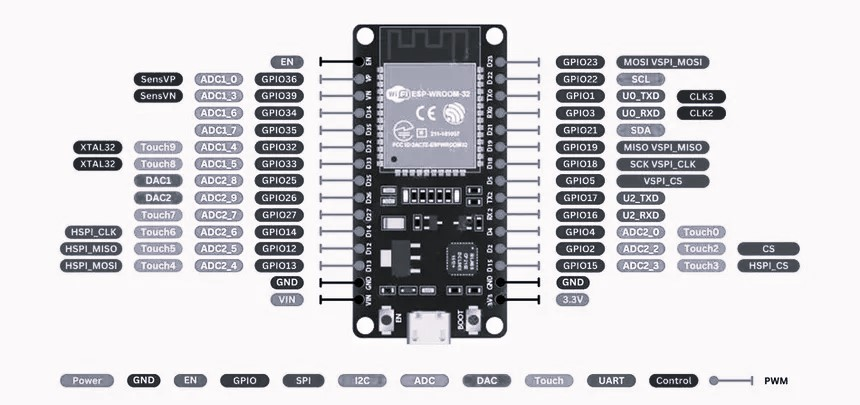
\includegraphics[width=0.5\linewidth]{img/esp32_pinout.png}
    \caption{Pinout do ESP32.}
    \label{fig:esp32-pinout}
\end{figure}

Para terminar, vamos conectar os pinos do ESP32 à protoboard. Escolhemos os pinos 18, 19 e 21 para o terminal vermelho, verde e azul do LED RGB, respectivamente. Utilizamos três cabos macho-fêmea para conectar os pinos aos pontos que estão conectados ao terminal do resistores. Usamos o último cabo para conectar o GND do ESP32 à linha negativa da protoboard, onde está conectado o terminal do cátodo do LED RGB.

\begin{figure}[H]
    \centering
    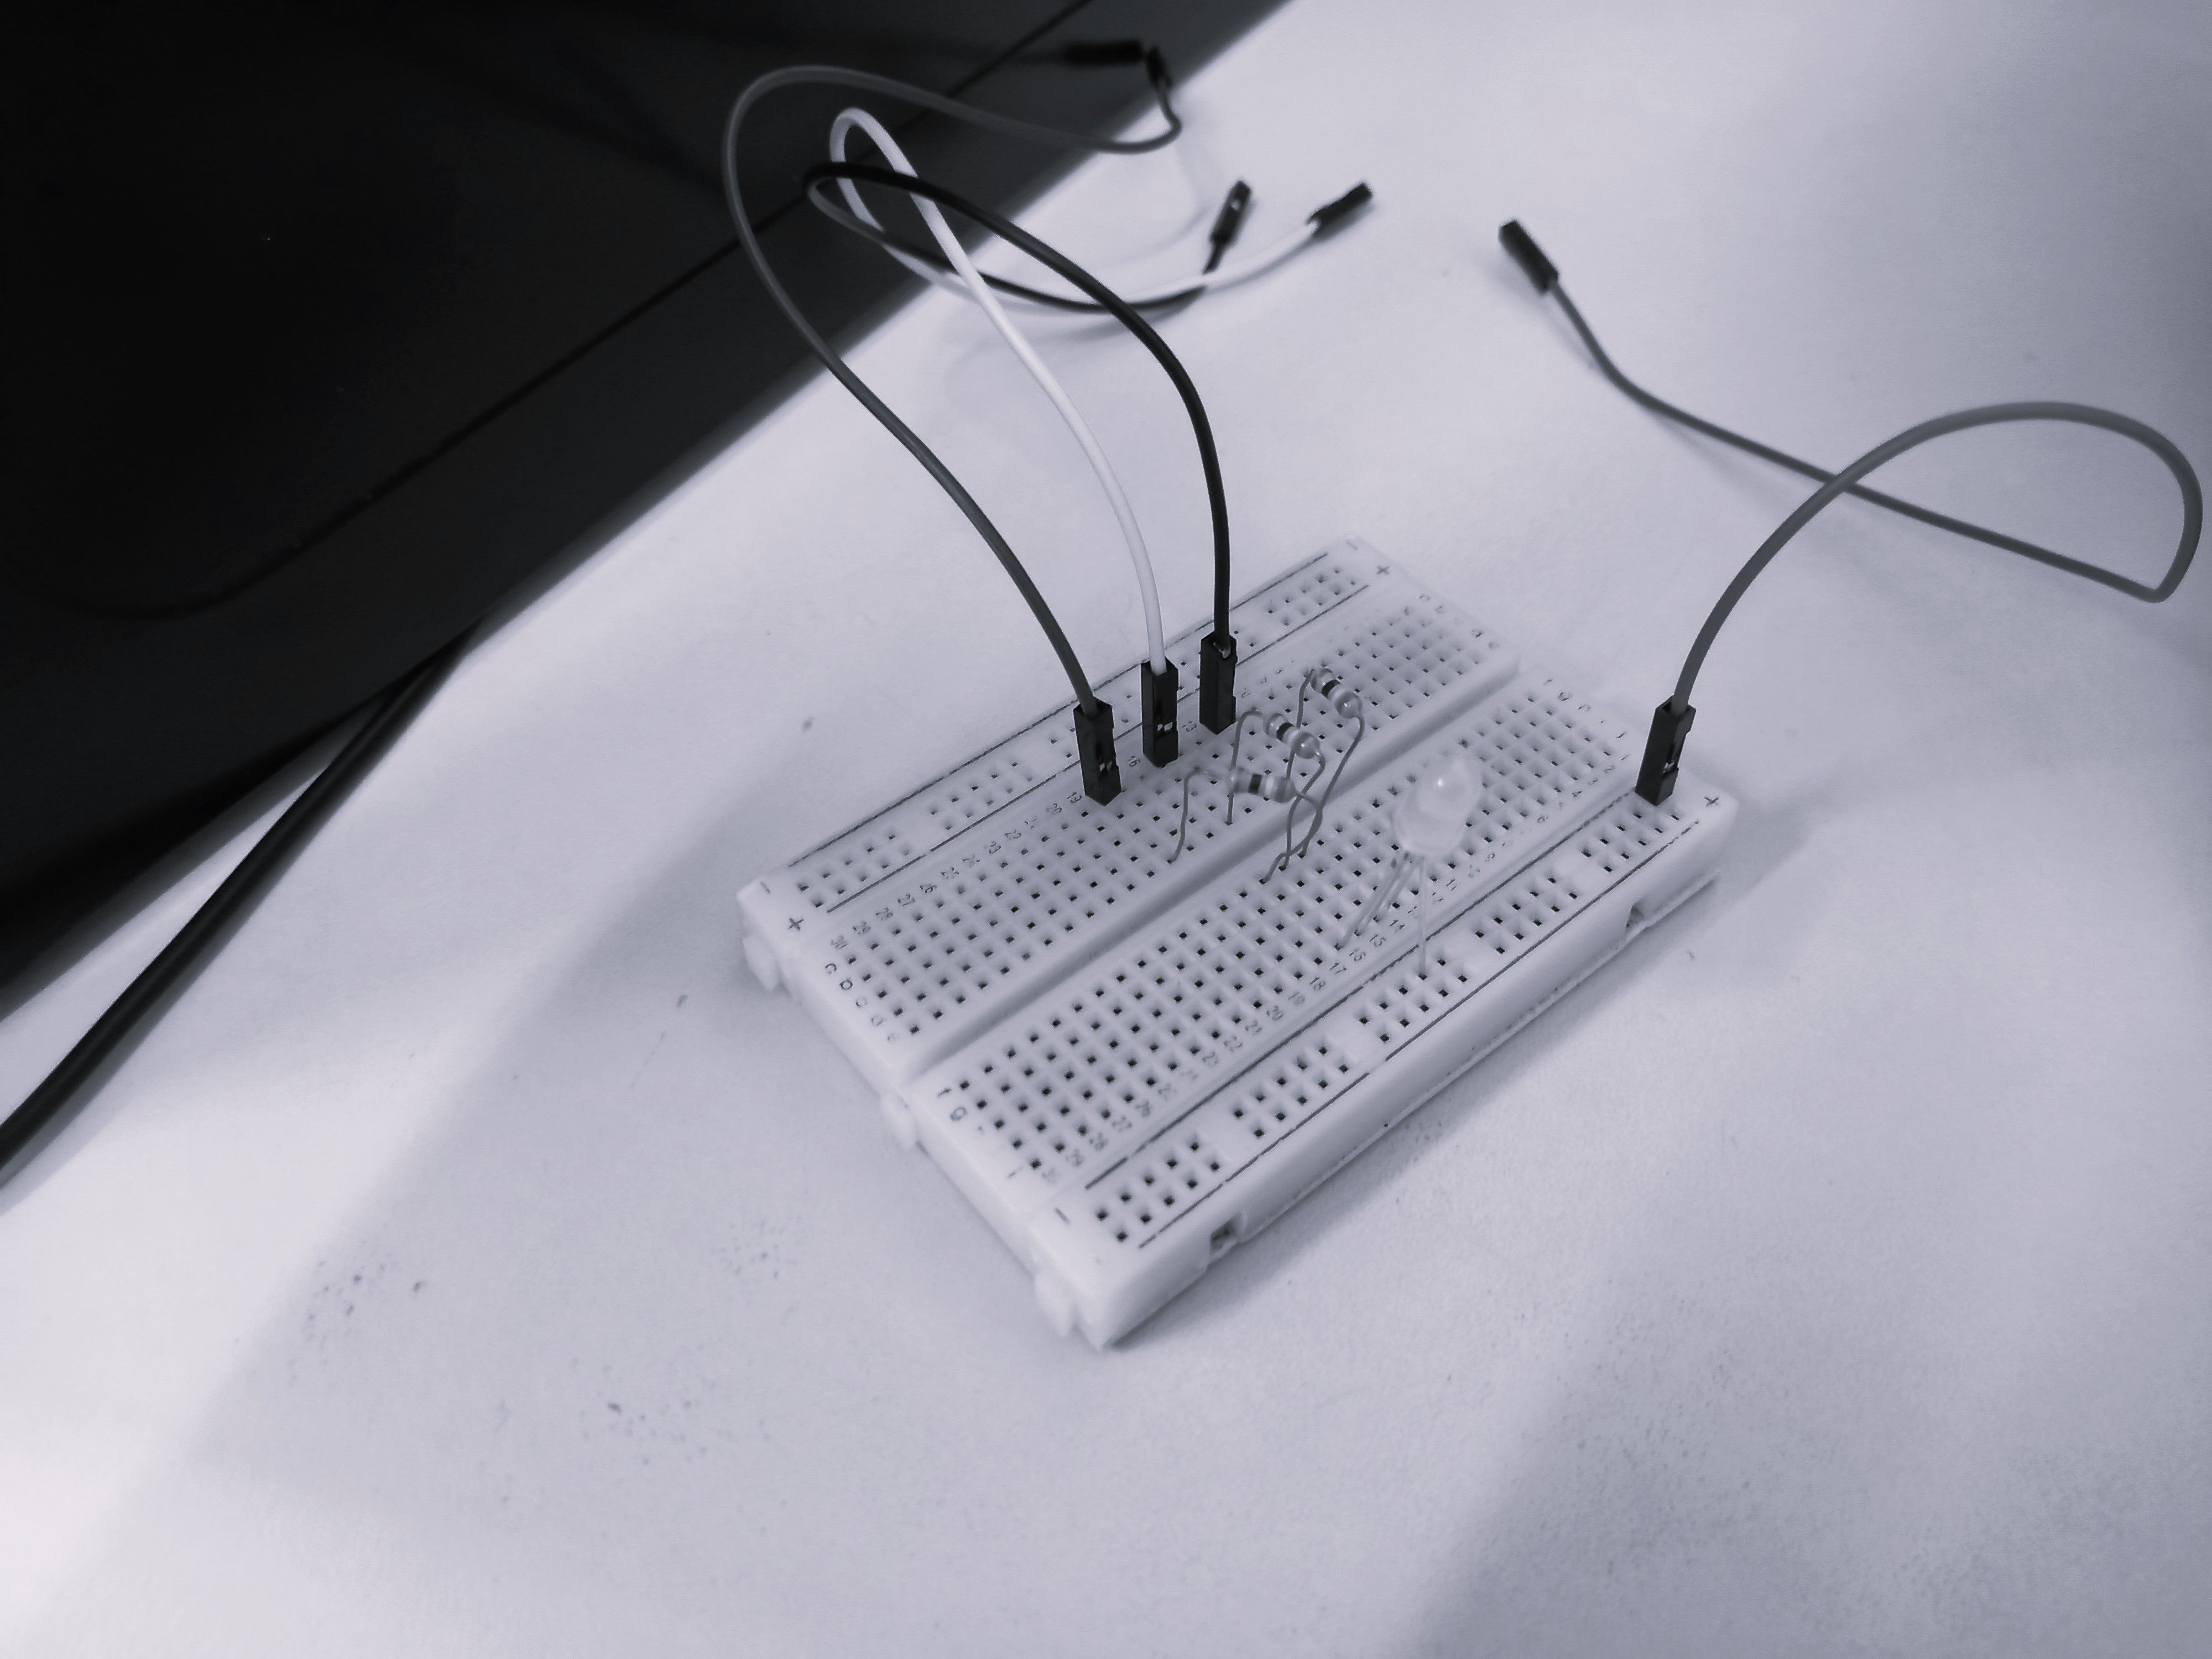
\includegraphics[width=0.5\linewidth]{img/20241125_095139.jpg}
    \caption{Configuração final.}
    \label{fig:final-config}
\end{figure}

\section{Servidor MQTT}

Acessamos o site \href{https://testclient-cloud.mqtt.cool/}{testclient-cloud.mqtt.cool} para nos conectamos a algum servidor \textit{MQTT} público para que possamos testar a nossa aplicação futuramente.

Escolhendo um servidor para conectar, aparece uma tela que se divide em \textit{Subscriptions} para criar tópicos, \textit{Publish} para publicar mensagens, e \textit{Messages} para mostrar as mensagens enviadas e recebidas.

Por agora, criamos os tópicos \textit{led\_algum} e \textit{mensagem\_alguma}. O tópico \textit{led\_algum} será usado para enviar e receber a cor do LED RGB. As mensagens precisam ser "red", "green" ou "blue" para fazer algum efeito. O tópico \textit{mensagem\_alguma} apenas recebe qualquer mensagem para imprimir no monitor.

\textit{QoS} signica \textit{Quality of Service}. Ele define qual o nível de conexão entre as máquinas. Se for \textit{QoS} 0, a entrega é de melhor esforço; se for \textit{QoS} 2, acontece um \textit{handshake} de quatro etapas. Depende muito da situação. Ficamos com \textit{QoS} 0 por ser um pequeno teste.

\begin{figure}[H]
    \centering
    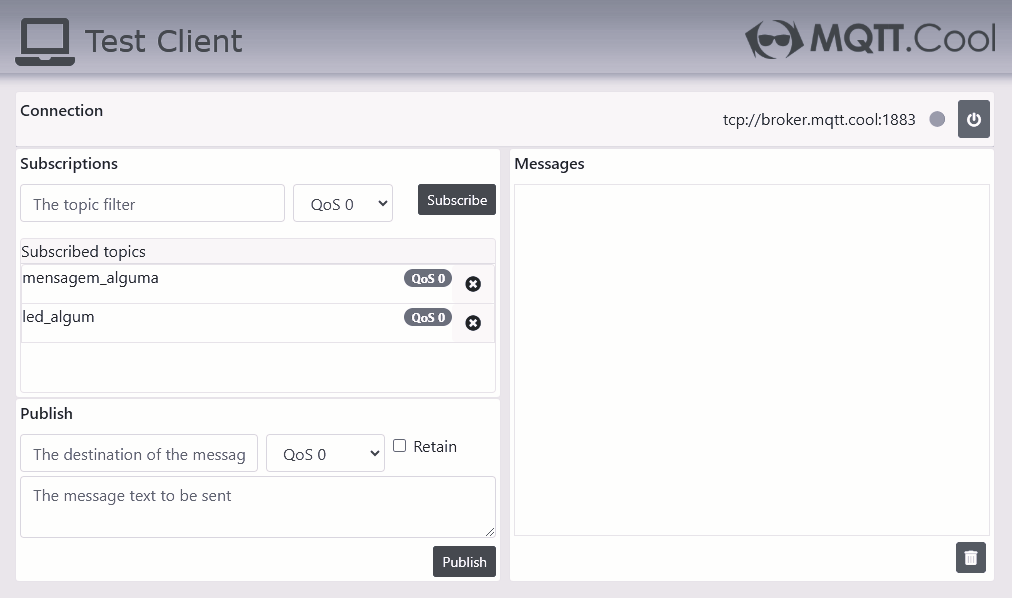
\includegraphics[width=0.5\linewidth]{img/Captura de tela 2024-11-26 231054.png}
    \caption{Tela do site MQTT.Cool.}
    \label{fig:mqtt-cool}
\end{figure}

\section{Desenvolvimento do Código}

Começamos criando um novo projeto pela página inicial do \textit{PlatformIO} no \textit{VSCode}. Com o título \textit{mqtt}, definindo a placa como \textit{Espressif ESP32 Dev Module} e utilizando o \textit{framework Arduino}. Depois de criado, voltando à página do PlatformIO e acessamos a \textit{Libraries} para instalar a biblioteca \textit{PubSubClient}. Adicionamos ela ao projeto e importamos no cabeçalho.

\lstinputlisting[language=C++, firstline=1, lastline=2]{code/main.cpp}

Definimos contantes para representar o número dos pinos do LED RGB e o SSID e a senha da rede a qual iremos conectar o ESP32 para que ele possa receber e enviar mensagens pela internet.

\lstinputlisting[language=C++, firstline=14, lastline=16]{code/main.cpp}

\lstinputlisting[language=C++, firstline=4, lastline=5]{code/main.cpp}

Na função \textit{setup}, iniciamos a \textit{Serial} com uma taxa de 9600, e também iniciamos o módulo \textit{WiFi} com o método \textit{begin}, passamos o SSID e a senha da rede como parâmetros. Colocamos um laço \textit{while} para que só saia quando o método \textit{status} confirme que a conexão foi realizada. Aproveitamos para configurar o modo dos pinos do LED utilizando a função \textit{digitalWrite}.

\lstinputlisting[language=C++, firstline=21, lastline=21]{code/main.cpp}

\lstinputlisting[language=C++, firstline=26, lastline=31]{code/main.cpp}

\lstinputlisting[language=C++, firstline=38, lastline=40]{code/main.cpp}

Para realizar a conexão com servidor \textit{MQTT}, definimos constantes para o endereço do servidor e para o número de porta. Agora, instanciamos um objeto da classe \textit{WifiClient} para passarmos ele no construtor da classe \textit{PubSubClient}, que é o objeto por onde enviamos e recebemos as mensagens. 

\lstinputlisting[language=C++, firstline=10, lastline=11]{code/main.cpp}

Voltando à função \textit{setup}, utilizamos o método \textit{setServer} do objeto recém-criado para definirmos qual é o servidor \textit{MQTT} que iremos conectar, passando como parâmetros o endereço e a porta que defininmos como constantes. Também utilizando a função \textit{setCallback} e passamos como parâmetro a função que realizará o \textit{callback}.

\lstinputlisting[language=C++, firstline=35, lastline=36]{code/main.cpp}

A função de \textit{callback} será executada toda vez que o servidor receber mensagem. A função recebe como parâmetros o nome do tópico das mensagem, a mensagem em sí e o tamanho da mensagem. A mensagem vem em formato de um ponteiro \textit{byte}, e por isso, utilizamos um laço para converter a mensagem para String.

\lstinputlisting[language=C++, firstline=44, lastline=44]{code/main.cpp}

\lstinputlisting[language=C++, firstline=48, lastline=53]{code/main.cpp}

Usamos \textit{ifs} condicionais para conduzir o fluxo dependendo do tópico. Se for o tópico \textit{mensagem\_alguma}, que é o mais simples, apenas imprimimos a mensagem no monitor com o método \textit{println} do \textit{Serial}. 

\lstinputlisting[language=C++, firstline=78, lastline=82]{code/main.cpp}

E se o tópico for \textit{led\_algum}, o conteúdo da mensagem servirá para definir qual será a cor do LED RGB, e para isso, usamos novamente \textit{ifs} condicionais. \newpage

\lstinputlisting[language=C++, firstline=56, lastline=76]{code/main.cpp}

Para finalizar, definimos uma função \textit{reconnect} que irá executar toda que o cliente \textit{MQTT} não estiver conectado. Dentro da função, há um laço \textit{while} que a sua condição de parada é que a conexão tenha sido realizada. A cada iteração, ele tenta realizar a conexão utilizando o método \textit{connect} do cliente, que retorna um valor \textit{booleano}. Quando for positivo, realizamos a inscrição de cada tópico dos quais queremos receber mensagem utilizando a função \textit{subscribe}.

\lstinputlisting[language=C++, firstline=85, lastline=99]{code/main.cpp}

Na função \textit{loop}, chamamos a função \textit{reconnect} toda vez que não houver conexão (sabemos utilizando o método do \textit{connected} do cliente). Também em \textit{loop}, usamos o método \textit{loop} do cliente para que ele processe as mensagens do servidor e mantenha a conexão.

\lstinputlisting[language=C++, firstline=101, lastline=106]{code/main.cpp}

É possível conferir o código completo nesse \href{https://github.com/fabricio-araujo94/microcontroladores/tree/main/mqtt}{repositório no GitHub}.

\section{Considerações Finais}

Feito tudo isso, conectamos o ESP32 ao computador utilizando o cabo microUSB, e por meio do atalho \textit{ALT + CTRL + U}, enviamos o código para o microcontrolador. Em certos casos, pode ser que seja necessário apertar o botão de \textit{boot} enquanto o código está sendo enviado ou após o código ter sido enviado.

Acessamos o site \href{https://testclient-cloud.mqtt.cool/}{testclient-cloud.mqtt.cool} e conectamos ao mesmo servidor que escolhemos ao escrever o código. Em \textit{Publish}, especificamos qual o tópico, o seu \textit{QoS} e a mensagem que queremos enviar. Em caso de não haver resposta, experimente outros servidores.

O vídeo demonstrando a prática pode ser acessado \href{https://youtu.be/7XPd-Q4VpAU}{aqui}.

\end{document}